\documentclass[a4paper]{article}
\usepackage[left=2cm, right=2cm, bottom=2.5cm, top=2.5cm]{geometry}
\usepackage[utf8]{inputenc}
\usepackage{amsmath}
\usepackage{amsfonts}
\usepackage{amssymb}
\usepackage{commath}
\usepackage{lipsum}
\usepackage{adjustbox}
\usepackage{float}
\usepackage{hyperref}
\usepackage{graphicx}
\usepackage{gensymb}
\usepackage[spanish]{babel}



\title{\Huge{\vspace{-1em}Resumen FVV1}}
\author{\Large{\vspace{-1em}Alex Mart\'inez Ascensi\'on}}
\makeatletter
\let\newtitle\@title
\let\newauthor\@author
\makeatother

\usepackage{xcolor}

\usepackage{wrapfig}

\usepackage{fancyhdr}
\pagestyle{fancy}
\lhead{Alex Martínez Ascensión}
\chead{}
\rhead{\today}


\usepackage[T1]{fontenc}
\usepackage[default]{gillius}

\setlength{\parskip}{1em}
\setlength{\parindent}{0em}

\newcommand{\dd}{\ensuremath{\operatorname{d}}}
\renewcommand{\d}[1]{\ensuremath{\operatorname{d}\!{#1}}}

\begin{document}
	\maketitle
	

\section{La geometría del espacio euclidiano}
\subsection{Vectores en el espacio tridimensional}
Un punto/vector se puede representar en el espacio real tridimensional, $\mathbb{R}^3$ como una tupla $(x,y,z)$ o de la forma $x\textbf{i}+y\textbf{j}+z\textbf{k}$, con $\textbf{i}, \textbf{j}$ y $\textbf{k}$ los vectores unitarios en la base canónica en $\mathbb{R}^3$: $(1,0,0), (0,1,0)$ y $(0,0,1)$. 

Si queremos representar una recta que pase por dos puntos $\textbf{a} = (x,y,z)$ y $\textbf{b} = (x', y', z')$, entonces tomamos el vector resta $\textbf{b}-\textbf{a}$ y la ecuación de la recta resultante es \[r(t) = \textbf{a} + t(\textbf{b}-\textbf{a})\]

\subsection{El producto interno}
Si tenemos dos vectores $\textbf{u}$ y $\textbf{v}$, ambos con la misma dimensión, entonces podemos aplicar la operación \textit{producto interno} o \textit{producto escalar}, definida como \textbf{$\cdot$} o $\langle\cdot,\cdot\rangle$: \[\langle\textbf{u},\textbf{v}\rangle=\textbf{u}\cdot \textbf{v}=u_1v_1+u_2v_2+\cdots+u_kv_k\] 
El producto interno cumple que es $\ge0$ y que es conmutativo ($\textbf{u}\cdot \textbf{v}=\textbf{v}\cdot\textbf{u}$). Además, también es asociativo $a\textbf{u}\cdot\textbf{v} = a(\textbf{u}\cdot\textbf{v}) = \textbf{u}\cdot a\textbf{v}$ y distributivo ($\textbf{a}\cdot(\textbf{u}+\textbf{v}) = \textbf{a}\cdot \textbf{u}+\textbf{a}\cdot \textbf{v}$)

Por otra parte, la norma de un producto, $\Vert\cdot\Vert$, queda definida como la raíz del producto escalar de un vector consigo mismo:
\[\Vert \textbf{a} \Vert = (\textbf{a}\cdot\textbf{a})^{1/2} \]
Así, en relación, $\Vert \textbf{a} \Vert^2= \textbf{a}\cdot\textbf{a} $

Dados dos vectores, $\textbf{u}$ y $\textbf{v}$, podemos definir el ángulo entre ellos con la siguiente relación: \[ \textbf{u} \cdot \textbf{v} = \Vert\textbf{u}\Vert \Vert\textbf{v}\Vert \cos\theta \]
Si el ángulo entre ambos vectores es de $90\degree$, entonces el producto interno es cero y, en tal caso, decimos que $\textbf{u}$ y $\textbf{v}$ son ortogonales.

Esta relación puede obtenerse desde la ley de los cosenos: $\Vert\textbf{u-v}\Vert^2=\Vert\textbf{v}\Vert^2+\Vert\textbf{u}\Vert^2-2\Vert\textbf{v}\Vert\Vert\textbf{u}\Vert\cos\theta$

Dos desigualdades claves en cálculo, usadas frecuentemente, son la \textit{desigualdad del triángulo} y la \textit{desigualdad de Cauchy-Schwarz} (izquierda y derecha):
\[\Vert\textbf{u}+\textbf{v}\Vert\le\Vert\textbf{u}\Vert+\Vert\textbf{v}\Vert \qquad\qquad |\textbf{u}\cdot\textbf{v}| \le \Vert\textbf{u}\Vert\Vert\textbf{v}\Vert \]

Por último, dados dos vectores, $\textbf{a}$ y $\textbf{c}$, la proyección de $\textbf{c}$ en $\textbf{a}$ es:\[ \text{proy}_\textbf{a}(\textbf{c}) = \textbf{a}\frac{\textbf{c}\cdot\textbf{a}}{\textbf{a}\cdot\textbf{a}} = \textbf{a}\frac{\textbf{c}\cdot\textbf{a}}{\Vert\textbf{a}\Vert^2}\]

\subsection{El producto en cruz}
Dados dos vectores $\textbf{u}$ y $\textbf{v}$, podemos definir la operación \textit{producto cruz} ($\times$) en $\mathbb{R}^3$ como:
\[ \textbf{u} \times \textbf{v} =\left| \begin{matrix}
\textbf{i} & \textbf{j} & \textbf{k}\\
u_1 & u_2 & u_3\\
v_1 & v_2 & v_3\\
\end{matrix}\right| \]

Así, el vector resultante es ortogonal tanto a \textbf{u} como a \textbf{v}, siguiendo la regla de la mano derecha. Podemos extender el producto en cruz de modo que el vector resultante sea multiplicado escalarmente con otro vector, $\textbf{w}$, de modo que así se crea el producto mixto:
\[ \textbf{w}\cdot(\textbf{u} \times \textbf{v}) =\left| \begin{matrix}
w_1 & w_2 & w_3\\
u_1 & u_2 & u_3\\
v_1 & v_2 & v_3\\
\end{matrix}\right| \]
La noción geométrica del producto mixto es que el determinante resultante es igual al volumen generado por los tres vectores a multiplicar. Asimismo, si tenemos dos vectores en $\mathbb{R}^2$, el determinante es el valor del área del paralelogramo que forman.

\rule{\linewidth}{1pt}

Una aplicación geométrica del producto escalar está en determinar ecuaciones de planos que cumplen ciertas condiciones. Un plano en $\mathbb{R}^3$ viene definido como el conjunto de puntos que satisfacen la ecuación $Ax+By+Cz=D$, de modo que $A, B, C $ y $D$ determinan la morfología del plano. Si $D=0$ el plano estará centrado en el origen.

\begin{wrapfigure}{r}{0pt}
		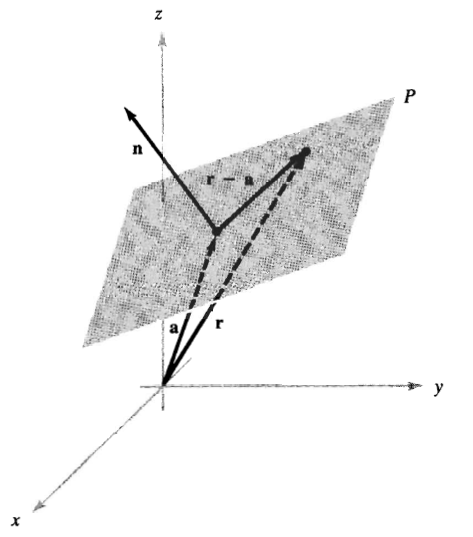
\includegraphics[width=0.35\linewidth]{./imagenes/ran.PNG}
\end{wrapfigure}

Buscamos un plano $P$ que contenga a todo $\textbf{r}$ en $P$ y que $\textbf{a}$ también sea un punto fijo de $P$. Además, como restricción imponemos que $P$ sea perpendicular a un vector $\textbf{n}$. Por tanto, $\textbf{n}$ también va a ser perpendicular a cualquier vector $\textbf{r}-\textbf{a}$. Si $\textbf{a} = (a_1, a_2, a_3), \textbf{n} = (A, B, C)$ y $\textbf{r}=(x,y,z)$, entonces la ecuación del plano nos queda: \[(\textbf{r}-\textbf{a})\cdot\textbf{n} = 0 \iff A(x-a_1)+B(y-a_2)+C(z-a_3)=0\]
Si ponemos que $D = -(Aa_1+Ba_2+Ca_3)$, entonces ya tenemos la ecuación del plano.

Por otra parte, la distancia entre un punto $\textbf{e}$ y un plano $P\equiv Ax+By+Cz=D$ es:
\[ d(\textbf{e}, P) = \frac{|Ae_1+Be_2+Ce_3+D|}{\sqrt{A^2+B^2+C^2}} \]

\subsection{Coordenadas esféricas y cilíndricas}

Si trabajamos en $\mathbb{R}^2$, podemos aplicar la transformación
\[ x = r\cos\theta \qquad \qquad y = r \sin\theta \]

Las coordenadas cilíndricas ($r$,$\theta$, $z$) vienen dadas por la transformación
\[ x = r\cos\theta \qquad \qquad y = r \sin\theta \qquad\qquad z= z \]

También podemos obtener la información explícitamente
\[ r = \sqrt{x^2+y^2} \qquad \qquad z = z \qquad\qquad \theta = \begin{cases}
\tan^{-1} (y/x) &\quad x > 0 \;\;y>0\\
\pi + \tan^{-1} (y/x) &\quad x < 0 \\
2\pi + \tan^{-1} (y/x) &\quad x > 0 \;\;y<0\\
\end{cases} \]


Las coordenadas cilíndricas ($\rho$,$\theta$, $phi$) vienen dadas por la transformación
\[ x = \rho\sin\phi\cos\theta \qquad \qquad y = \rho\sin\phi\sin\theta \qquad\qquad z = \rho\cos\phi \]

\begin{figure}[h!]
	\centering
	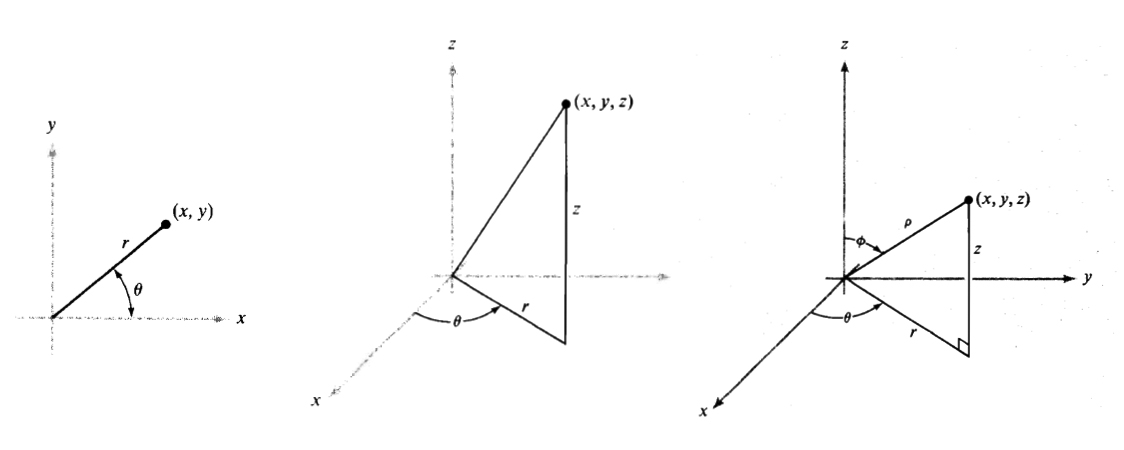
\includegraphics[width=0.87\linewidth]{./imagenes/coords.jpg}
\end{figure}

\section{Diferenciación}
\subsection{Geometría de las funciones con valores reales}
Sea $f:U\subset\mathbb{R}^n\rightarrow\mathbb{R}$ y sea $c \in \mathbb{R}$. Entonces el conjunto de nivel de $c$ se define como todos los puntos $\textbf{x}\in U$ para los que $f(\textbf{x})=c$. Si $n=2$, hablamos de una curva de nivel y si $n=3$ se trata de una superficie de nivel. 

Así, por ejemplo, la esfera $x^2+y^2+z^2=1$ puede describirse como un grupo de curvas de nivel de modo que $c = 1-z^2$ y resolvemos las ecuaciones $x^2 + y^2 = c$ para varios valores de $z \in [-1,1] \rightarrow c \in [0, 1] $. 

\begin{figure}[h!]
	\centering
	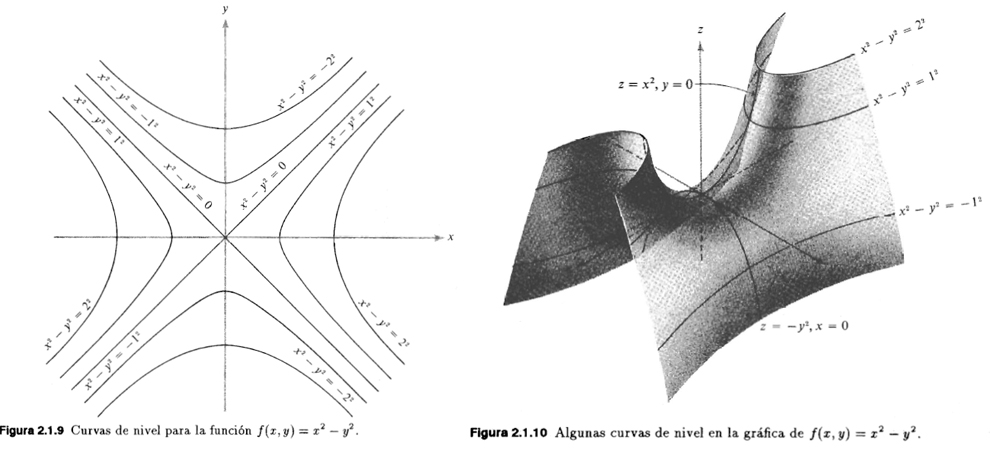
\includegraphics[width=0.87\linewidth]{./imagenes/curvas.jpg}
\end{figure}

Otro ejemplo es el de la imagen de arriba, la función $f(x,y) = x^2-y^2$. Tomamos diferentes valores de $z=f(x,y)$ y graficamos.

\subsection{Límites y continuidad}
Sea $U\subset\mathbb{R}^n$. Decimos que un conjunto es abierto cuando para cualquier punto $\textbf{x}_0$ en $U$ existe algún $r>0$ tal que $D_r(\textbf{x}_0) = \{\textbf{x}:\Vert\textbf{x}-\textbf{x}_0\Vert<r\}$ está contenido en $U$. Por otra parte, un punto $\textbf{x}$ es un punto frontera en $U$ si todo $D_r(\textbf{x})$ tiene por lo menos un punto perteneciente a $U$ y otro no perteneciente.

El concepto de límite para varias variables es igual que para el de una variable, sólo que cambia el concepto de bola o vecindad para varias variables. Las propiedades de los límites para una función $f:A\subset\mathbb{R}^n \rightarrow \mathbb{R}^m$ son las siguientes:
\begin{itemize}
	\item Si $\lim_{\textbf{x}\rightarrow\textbf{x}_0} f(\textbf{x}) = \textbf{b}$ entonces $\lim_{\textbf{x}\rightarrow\textbf{x}_0} cf(\textbf{x}) = c\textbf{b}$
	\item Si $\lim_{\textbf{x}\rightarrow\textbf{x}_0} f(\textbf{x}) = \textbf{b}_1$ y   $\lim_{\textbf{x}\rightarrow\textbf{x}_0}g(\textbf{x}) = \textbf{b}_2$ entonces $\lim_{\textbf{x}\rightarrow\textbf{x}_0} (f+g)(\textbf{x}) = \textbf{b}_1+\textbf{b}_2$
		\item Si\textbf{ m=1} y $\lim_{\textbf{x}\rightarrow\textbf{x}_0} f(\textbf{x}) = \textbf{b}_1$ y   $\lim_{\textbf{x}\rightarrow\textbf{x}_0}g(\textbf{x}) = \textbf{b}_2$ entonces $\lim_{\textbf{x}\rightarrow\textbf{x}_0} (fg)(\textbf{x}) = \textbf{b}_1\textbf{b}_2$
	\item Si\textbf{ m=1} y $\lim_{\textbf{x}\rightarrow\textbf{x}_0} f(\textbf{x}) = \textbf{b}\neq0$ y $f(\textbf{x})\neq0$ entonces $\lim_{\textbf{x}\rightarrow\textbf{x}_0} 1/f(\textbf{x}) = 1/\textbf{b}$
	\item Si $f(\textbf{x})=(f_1(\textbf{x}),\cdots,f_m(\textbf{x}))$ entonces $\lim_{\textbf{x}\rightarrow\textbf{x}_0}f(\textbf{x})=\textbf{b}=(b_1,\cdots,b_m)$ sii $\lim_{\textbf{x}\rightarrow\textbf{x}_0}f_i(\textbf{x})=b_i$
\end{itemize}

Una función $f$ es continua en $\textbf{x}_0$ sii $\lim_{\textbf{x}\rightarrow\textbf{x}_0}f(\textbf{x}) = f(\textbf{x}_0)$. Los cinco puntos de propiedades de límites son también aplicables a continuidad.

La composición de funciones también es continua. Es decir, si tenemos dos funciones $f:B\subset\mathbb{R}^m\rightarrow\mathbb{R}^p$ y $g:A\subset\mathbb{R}^n\rightarrow\mathbb{R}^m$, si se cumple que $g$ es continua en $\textbf{x} \in A$ y $f$ es continua en $g(\textbf{x})$, entonces $(f \circ g)(\textbf{x}) = f(g(\textbf{x}))$ también es continua en $\textbf{x}$.

Cuando queremos resolver un límite multivariable [$\lim_{(\textbf{x})\rightarrow(\textbf{x}_0)} f(\textbf{x}) = \textbf{b}$] podemos emplear varias estrategias:
\begin{itemize}
	\item Si tenemos imaginación, y a veces cuando no queda otra, recurrimos a la notación $\delta-\epsilon$ para demostrar que para todo $\delta>0$ existe un $\epsilon>0$ tal que si $\Vert\textbf{x}- \textbf{x}_0\Vert < \delta$, entonces $\Vert f(\textbf{x}) - \textbf{b}\Vert < \epsilon$. Sin embargo, cada caso es excepcional, y puede no ser fácilmente demostrable.
	\item Podemos probar a emplear límites iterados, es decir, para $\textbf{x} = (x_1,\cdots, x_m)$, podemos tomar $x_1$ como variable y el resto como constantes, y así ir repitiendo el límite: $\lim_{\textbf{x}\rightarrow\textbf{a}} f(\textbf{x}) = \lim_{\textbf{x}_1\rightarrow\textbf{a}_1} (\lim_{\textbf{x}_2\rightarrow\textbf{a}_2}(\cdots ( \lim_{\textbf{x}_n\rightarrow\textbf{a}_n}f(\textbf{x}))))$ e ir repitiendo con otras combinaciones ($ \lim_{\textbf{x}_2\rightarrow\textbf{a}_2} (\lim_{\textbf{x}_4\rightarrow\textbf{a}_4}(\cdots ( \lim_{\textbf{x}_1\rightarrow\textbf{a}_1}f(\textbf{x}))))$). Si en alguno de los casos un límite difiere, entonces tenemos que el límite no existe. Sin embargo, si en todos los casos los límites existen y son iguales, NO PODEMOS DECIR QUE EL LÍMITE EXISTA.
	\item Podemos aproximarnos al límite desde diferentes trayectorias ($x=0$, $y=x$, $y=x^2-z$) y buscar una trayectoria para la cual el límite sea diferente del resto. En este caso, probar que el límite exista en una trayectoria no demuestra que el límite exista, ya que deberíamos probar todas las trayectorias posibles.
	\item Podemos pasar el límite a coordenadas polares / esféricas y ver qué pasa. 
	\end{itemize}

\subsection{Diferenciación}

Recordamos el concepto de derivada en punto para funciones de una variable. Decimos que una función $f$ es derivable en $a$ cuando existe el límite
\[f'(a) = \lim_{x\rightarrow a}\frac{f(x)-f(a)}{x-a} = \lim_{h\rightarrow 0}\frac{f(a+h)-f(a)}{h}\]
Y decimos que $f$ es derivable en general cuando lo es para todos los puntos de $\mathbb{R}$

En este caso, para funciones de varias variables aplicamos el concepto de derivada parcial, de modo que la derivada queda definida de la siguiente manera:
\[ \frac{\partial f}{\partial x_j}(x_1,\cdots,x_n) = \lim_{h\rightarrow 0}\frac{f(x_1,x_2,\cdots,x_j+h,\cdots,x_n) - f(x_1,x_2,\cdots,x_j,\cdots,x_n)}{h} \]
Este caso es aplicable para $f:\mathbb{R}^n\rightarrow\mathbb{R}$. En el caso de $f:\mathbb{R}^n\rightarrow\mathbb{R}^m$, hablaríamos de $\frac{\partial f_k}{\partial x_j}$ a la parcial de la k-ésima funcion para la j-ésima variable.

Las derivadas de una función para todas las variables se resume en la matriz de la derivada de $f$:
\[\textbf{D}f(\textbf{x}_0) = \left[\begin{matrix}
\frac{\partial f_1}{\partial x_1} & \cdots & \frac{\partial f_1}{\partial x_n}\\
\vdots & & \vdots\\
\frac{\partial f_m}{\partial x_1} & \cdots & \frac{\partial f_m}{\partial x_n}\\
\end{matrix}\right]  \]
Esta matriz también se llama \textbf{\textit{matriz jacobiana}} o \textit{\textbf{diferencial jacobiana}}.

Dicho esto, más precisamente, tenemos que $f$ es diferenciable en $\textbf{x}_0$ si
\[ \lim_{\textbf{x}\rightarrow \textbf{x}_0}\frac{\Vert f(\textbf{x}) - f(\textbf{x}_0)-\textbf{D}f(\textbf{x}_0)(\textbf{x}-\textbf{x}_0)\Vert}{\Vert\textbf{x}-\textbf{x}_0\Vert} = 0 \]

Cuando $\textbf{D}f(\textbf{x}) = \left[\begin{matrix}
\frac{\partial f}{\partial x_1} & \cdots & \frac{\partial f}{\partial x_n}\\ 
\end{matrix}\right]  $ entonces simplificamos la notación de matriz derivada a gradiente de $f$, $\nabla f$. 

Finalmente, podemos extrapolar el concepto de diferenciabilidad para todo $\textbf{x}$. Sea $f:U\subset \mathbb{R}^n \rightarrow \mathbb{R}^m$. Para que $f$ sea diferenciable en $x$ todas las derivadas parciales de $f$ han de existir y han de ser continuas en $\textbf{x}$. Esto último es clave: si alguna derivada parcial existe pero no es continua en $\textbf{x}$, entonces $f$ no es diferenciable. 

Si $f$ es k-diferenciable, entonces decimos que es del tipo $C^k$.


\subsection{Propiedades de la derivada}
Las propiedades comunes de una variable sobre suma y producto de derivadas se mantienen en el caso multivariable:
\begin{itemize}
	\item Si $h(\textbf{x}) = cf(\textbf{x})$, entonces $\textbf{D}h(\textbf{x}) = c\textbf{D}f(\textbf{x})$
	\item Si $h(\textbf{x}) = f(\textbf{x})+ g(\textbf{x})$, entonces $\textbf{D}h(\textbf{x}) = \textbf{D}f(\textbf{x})+\textbf{D}g(\textbf{x})$
	\item Si $h(\textbf{x}) = f(\textbf{x})g(\textbf{x})$, entonces $\textbf{D}h(\textbf{x}) = g(\textbf{x})\textbf{D}f(\textbf{x}) + f(\textbf{x})\textbf{D}g(\textbf{x})$
	\item Si $h(\textbf{x}) = f(\textbf{x})/g(\textbf{x})$, entonces $\textbf{D}h(\textbf{x}) = \frac{g(\textbf{x})\textbf{D}f(\textbf{x})-f(\textbf{x})\textbf{D}g(\textbf{x})}{[g(\textbf{x})]^2}$
\end{itemize}
Recordamos de cálculo de una variable que si tenemos una función $f(g(x))$, entonces la derivada es, aplicando la regla de la cadena: 
\[ \frac{\d f}{\d x} = \frac{\d f}{\d g}\frac{\d g}{\d x} = f'(g)g'(x) \]

En el caso de funciones multivariable se extiende el concepto tal que si, por ejemplo, $h = f(g(x),k(x),j(x))$ entonces 
\[\frac{\d h}{\d x} = \frac{\partial f}{\partial g}\frac{\d g}{\d x} + \frac{\partial f}{\partial k}\frac{\d k}{\d x} + \frac{\partial f}{\partial j}\frac{\d j}{\d x} = \left[\begin{matrix}
\frac{\partial f}{\partial g} & \frac{\partial f}{\partial j} & \frac{\partial f}{\partial k}
\end{matrix}\right]\left[\begin{matrix}
\frac{\d g}{\d x}\\ \frac{\d j}{\d x}\\ \frac{\d k}{\d x}\\
\end{matrix}\right] = \nabla f\cdot \textbf{D}h\]

$h = f(g(x,y,z),k(x,y,z),j(x,y,z))$ entonces $\nabla f$ es:
\[  \frac{\partial h}{\partial x} = \frac{\partial f}{\partial g}\frac{\partial g}{\partial x} + \frac{\partial f}{\partial k}\frac{\partial k}{\partial x} + \frac{\partial f}{\partial j}\frac{\partial j}{\partial x}\]
\[  \frac{\partial h}{\partial y} = \frac{\partial f}{\partial g}\frac{\partial g}{\partial y} + \frac{\partial f}{\partial k}\frac{\partial k}{\partial y} + \frac{\partial f}{\partial j}\frac{\partial j}{\partial y}\]
\[  \frac{\partial h}{\partial z} = \frac{\partial f}{\partial g}\frac{\partial g}{\partial z} + \frac{\partial f}{\partial k}\frac{\partial k}{\partial z} + \frac{\partial f}{\partial j}\frac{\partial j}{\partial z}\]

Así, 
\[\nabla h = \left[\frac{\partial h}{\partial x}, \frac{\partial h}{\partial y}, \frac{\partial h}{\partial z}\right] =  \left[\frac{\partial f}{\partial g}, \frac{\partial f}{\partial k}, \frac{\partial f}{\partial j}\right]  \left[\begin{matrix}
\frac{\partial g}{\partial x} & \frac{\partial g}{\partial y} & \frac{\partial g}{\partial z}\\
\frac{\partial k}{\partial x} & \frac{\partial k}{\partial y} & \frac{\partial k}{\partial z}\\
\frac{\partial j}{\partial x} & \frac{\partial j}{\partial y} & \frac{\partial j}{\partial z}\\
\end{matrix}\right] \rightarrow \nabla h = \nabla f \cdot \textbf{D}h \]


\subsection{Gradientes y derivadas direccionales}
Si $f:\mathbb{R}^3\rightarrow\mathbb{R}$, la derivada direccional de $f$ en $\textbf{x}$ en la dirección de un vector $\textbf{v}$ está dada por 
\[ \left.\frac{\dd}{\d t} f(\textbf{x} + t\textbf{v}) \right|_{t=0} = \lim_{h \rightarrow 0} \frac{f(\textbf{x} + h\textbf{v})-f(\textbf{x})}{h}\]

Si tomamos $c(t) = \textbf{x} + t\textbf{v}$, entonces $\frac{\dd}{\d t} f(c(t)) = \nabla f(c)\cdot c'(t)$. Como $c(0) = \textbf{x}$ y $c'(t) = \textbf{v}$, entonces la derivada direccional es $\left.\frac{\dd}{\d t} f(\textbf{x} + t\textbf{v}) \right|_{t=0} = \nabla f(\textbf{x})\cdot \textbf{v}$.

Como visión geométrica, tenemos que el gradiente apunta en la dirección normal al plano tangente de la superficie de la gráfica en el punto. Asimismo, el gradiente también apunta en la dirección en la que $f$ crece más rápido. Por ende, el negativo del gradiente indica la dirección en la que $f$ decrece más rápido. 

Por tanto, si $\textbf{v}$ es el vector tangente de una trayectoria $c(t)$ de una superficie $S$ en $t=0$, entonces el gradiente de la función $f$ en ese será ortogonal a $\textbf{v}$, es decir, $\nabla f(c(0)) \cdot \textbf{v} = 0$.

Así, extendiendo lo que vimos en 2.3, el plano tangente a una superficie $S$ en un punto $(x_0,y_0,z_0)$ es $$P \equiv \nabla f \cdot (x-x_0,y-y_0,z-z_0) = 0$$

\subsection{Derivadas parciales iteradas}
Hasta la fecha hemos realizado sólo una diferenciación a las funciones, y hemos tratado con funciones $C^1$. Sin embargo, podemos diferenciar varias veces, de modo que podemos extender la notación de derivada parcial a una derivada parcial iterada:
\[ \frac{\partial^k f}{\partial x_1 \partial x_2 \cdot \partial x_k}  =
\frac{\partial}{\partial x_1} \left( \frac{\partial}{\partial x_2} \left( \cdots\left( \frac{\partial f}{\partial x_k}  \right)\right)\right) \qquad
\frac{\partial^k f}{\partial x^k}  =
\frac{\partial}{\partial x} \left( \frac{\partial}{\partial x} \left( \overset{k \text{ veces}}{\cdots}\left( \frac{\partial f}{\partial x}  \right)\right)\right)\] 

Si la función es $C^2$, el teorema de la derivada mixta afirma que 
\[ f_{yx} = \frac{\partial^2 f}{\partial x \partial y}  =  \frac{\partial^2 f}{\partial y \partial x} = f_{xy}\] 

Este concepto puede extenderse a funciones de cualquier tipo $C^k$.


\section{Funciones con valores vectoriales}
\subsection{Trayectorias y velocidad}
Una trayectoria es una función $\boldsymbol{\sigma}:[a,b] \rightarrow \mathbb{R}^n$. Los puntos $\boldsymbol{\sigma}(a)$ y $\boldsymbol{\sigma}(b)$ son los extremos de la trayectoria. La imagen de la trayectoria en $\mathbb{R}^n$ se llama curva. 

Así, una trayectoria $\boldsymbol{\sigma}(t)$ puede definirse en $\mathbb{R}^3$ como una función $\boldsymbol{\sigma}(t) = (x(t), y(t), z(t))$. La derivada de la trayectoria viene definida como:
\[ \boldsymbol{\sigma}'(t) = \lim_{h \rightarrow 0}\frac{\boldsymbol{\sigma}(t_0+h)-\boldsymbol{\sigma}(t_0)}{h} = (x'(t), y'(t), z'(t)) \]

La recta tangente a una trayectoria es $\textbf{l}(\lambda) = \boldsymbol{\sigma}(t_0) + \lambda\boldsymbol{\sigma}'(t_0)$

A nivel físico, si tenemos una trayectoria $\textbf{r}(t)$, a velocidad es $\textbf{v}(t)=\textbf{r}'(t)$, la rapidez es $S(t) = \Vert\textbf{v}(t)\Vert$ y la aceleración es $\textbf{a}(t) = \textbf{r}''(t)$.

\subsection{Longitud de arco}
Si tenemos una trayectoria $\boldsymbol{\sigma}:[a,b] \rightarrow \mathbb{R}^n$, la longitud de arco entre $a$ y $b$ está definida como:
\[ l(\boldsymbol{\sigma}) = \int^a_b{\Vert\boldsymbol{\sigma}'(t)\Vert \d t} = \int^a_b{\sqrt{ [x_1'(t)]^2+[x_2'(t)]^2+\cdots+[x_n'(t)]^2 }} \d t \]

Por lo general no nos interesa obtener la longitud de arco entre dos puntos, sino dado un $a$ fijo, obtener una función de longitud de arco para un tiempo $t$:
\[  s(t) = \int_a^t{\Vert\boldsymbol{\sigma}'(\tau)\Vert \d \tau} \]

Así, por el Primer Teorema del Cálculo, tenemos que $s'(t) = \Vert\boldsymbol{\sigma}'(t)\Vert$

\subsection{Campos vectoriales}
Un campo vectorial en $\mathbb{R}^n$ es una función $\textbf{F}: A  \subset \mathbb{R}^n \rightarrow \mathbb{R}^m$ que asigna a cada vector $\textbf{x}$ en $A$ su vector $\textbf{F}(\textbf{x})$ en $\mathbb{R}^m$. Así, por ejemplo, para una partícula posicionada en $\textbf{r}  =(x,y,z)$, su fuerza de atracción localizada en el origen es un campo vectorial $\textbf{F} = - \frac{mMG}{\Vert\textbf{r}\Vert^3}\textbf{r}$.

Una línea de flujo para $\textbf{F}$ es una trayectoria $\boldmath{\sigma}(t)$ tal que 
\[ \boldsymbol{\sigma}'(t) = \textbf{F}(\boldsymbol{\sigma}(t)) \]
Es decir, el argumento del campo vectorial es la propia trayectoria, y su imagen ha de ser igual a la derivada de la trayectoria. En condiciones iniciales, tomamos $\boldsymbol{\sigma}(0) = (x_0, y_0, z_0)$.

Para agilizar la notación, definimos $\phi(\textbf{x}, t)$ como la posición del punto en la línea de flujo tras haber transcurrido un tiempo $t$. Así, la ecuación anterior se reescribe como (además de una segunda condición inicial):
\[ \phi(\textbf{x}, 0) = \textbf{x} \qquad \frac{\partial}{\partial t} \phi(\textbf{x}, t)  \]

\subsection{Divergencia y rotacional de un campo vectorial}
Usualmente tomamos el gradiente como una función asociada a una función. Sin embargo, el gradiente como tal es un operador, es decir, un elemento matemático que combinado a una función modifica sus valores. Así, el gradiente como tal está definido como:
\[ \boldsymbol{\nabla}  = \textbf{i}\frac{\partial}{\partial x} + \textbf{j}\frac{\partial}{\partial y} + \textbf{k}\frac{\partial}{\partial z}\]

Y cuando hacemos $\nabla f$ en realidad hacemos el producto escalar entre $\boldsymbol{\nabla} $ y $f$.

La \textit{operación rotacional} asocia a cada campo vectorial $C^1$ $\textbf{F}$ el siguiente campo vectorial:
\[ \text{rot } \textbf{F} = {\boldsymbol{\nabla}} \times \textbf{F} = \left| \begin{matrix}
\textbf{i} & \textbf{j} & \textbf{k} \\
\frac{\partial}{\partial x} & \frac{\partial}{\partial y}  & \frac{\partial}{\partial z}  \\
F_1 & F_2 & F_3 \\
\end{matrix}\right| 
\]

Si ${\boldsymbol{\nabla}} \times \textbf{F}=0$, entonces decimos que $\textbf{F}$ es irrotacional.

Otra función es la \textit{divergencia} de un campo vectorial, definida como:
\[  \text{div } \textbf{F} = {\boldsymbol{\nabla}} \cdot \textbf{F} = \frac{\partial F_1}{\partial x} + \frac{\partial F_2}{\partial y} + \frac{\partial F_3}{\partial z} \]

En este campo, la divergencia es un campo escalar, a diferencia del rotacional, que es un campo vectorial.

Como "curiosidad", es importante recordar que la divergencia de un rotacional siempre es 0: 
\[ {\boldsymbol{\nabla}} \cdot ({\boldsymbol{\nabla}} \times \textbf{F}) = 0\] 

\rule{\linewidth}{1pt}

Además del operador gradiente existen otros muchos. Uno de los más importantes es el \textit{operador laplaciano}, definido como
\[ \Delta f = (\nabla\cdot\nabla)f = \nabla^2f = \sum^n_i\frac{\partial^2f}{\partial x_i^2} \]
Cuando una función cumple que su laplaciano es nulo, es decir, $\nabla^2f = 0$ decimos que es una \textit{función armónica}.
\section{Derivadas de orden superior; Máximos y mínimos}
\subsection{Teorema de Taylor}
Si recordamos el teorema para una variable, dada una función $f$ derivable $k$ veces en un punto $a$, entonces podemos escribir una aproximación de $f$ como:
\[ f(x) = f(a) + f'(a) (x-a) + \frac{f''(a)}{2!} (x-a)^2 + \cdots + \frac{f^{(k)}}{k!}(x-a)^k + R_k(x,a)\]
con $R_k$:
\[ R_k(x,a) = \int_a^x{\frac{(x-t)^k}{k!}f^{(k+1)}(t) \d t} \]

Así, conforme mayor es $k$, menor es $R_k$, y obtenemos una mejor aproximación de $f$.

Si desarrollamos el teorema para varias variables con derivadas hasta de tercer orden tenemos la expresión:
\[ f(\textbf{x}_0+\textbf{h}) = f(\textbf{x}_0) + \sum^n_i{h_i\frac{\partial f}{\partial x_i}(\textbf{x}_0)} + \frac{1}{2!} \sum^n_{i,j}{h_ih_j\frac{\partial f}{\partial x_i \partial x_j}(\textbf{x}_0)} + R_2(\textbf{h}, \textbf{x}_0) \]

Aquí cambiamos un poco la notación por conveniencia. Si definimos $\textbf{x} = \textbf{x}_0 + \textbf{h}$, entonces  $f(\textbf{x}_0+\textbf{h})$, donde $\textbf{x}_0$ sería el equivalente multidimensional de $a$, entonces $\textbf{h} = \textbf{x} - \textbf{x}_0$, que sería el equivalente multidimensional de $(x-a)$. Por tanto, la expresión final nos va a quedar en función de $\textbf{h}$.

La expresión anterior se puede expandir hasta el orden que deseemos, k:
\[ f(\textbf{x}_0+\textbf{h}) = f(\textbf{x}_0) + \sum^n_{m_1}{h_{m_1}\frac{\partial f}{\partial x_{m_1}}(\textbf{x}_0)} + \frac{1}{2!} \sum^n_{{m_1},{m_2}}{h_{m_1}h_{m_2}\frac{\partial^2 f}{\partial x_{m_1} \partial x_{m_2}}(\textbf{x}_0)} + \cdots \]\[+
 \frac{1}{k!} \sum^n_{{m_1},{m_2},\cdots,{m_k}}{h_{m_1}h_{m_2}\cdots h_{m_k}\frac{\partial^k f}{\partial x_{m_1} \partial x_{m_2} \cdots\partial x_{m_k}}(\textbf{x}_0)}
  + R_k(\textbf{h}, \textbf{x}_0) \]

\subsection{Extremos de funciones con valores reales}
Si $U \subset \mathbb{R}^n$ es abierto, $f: U \subset \mathbb{R}^n \rightarrow \mathbb{R}$ es diferenciable y $\textbf{x}_0 \in U$, entonces $\textbf{D}f(\textbf{x}_0)$ es un punto crítico de $f$. Por tanto, para hallar extremos críticos, realizamos la derivada de $f$ e igualamos a cero su matriz derivada. La condición que haga que todos los elementos de la matriz derivada sean 0 es un punto crítico.

Si suponemos que $f$ tiene derivadas de segundo orden, entonces el hessiano de $f$ en $\textbf{x}_0$ es:
\[ Hf(\textbf{x}_0)(\textbf{h}) = \frac{1}{2} \sum^n_{i,j}{h_ih_j\frac{\partial^2 f}{\partial x_i \partial x_j}(\textbf{x}_0)}\]

Esta expresión puede reescribirse en forma matricial como:
\[ H(\textbf{h}) = \frac{1}{2} \left[\begin{matrix}
h_1&h_2&\cdots &h_n
\end{matrix}\right] 
B
\left[\begin{matrix}
h_1\\h_2\\\cdots\\ h_n
\end{matrix}\right] \qquad \textbf{H} = B = \left[\begin{matrix}
\frac{\partial^2 f}{\partial x_1^2} & \frac{\partial^2 f}{\partial x_1 \partial x_2} &\cdots& \frac{\partial^2 f}{\partial x_1 \partial x_n} \\
\frac{\partial^2 f}{\partial x_2\partial x_1} & \frac{\partial^2 f}{ \partial x_2^2} &\cdots& \frac{\partial^2 f}{\partial x_2 \partial x_n} \\
\vdots & \vdots &\ddots& \vdots \\
\frac{\partial^2 f}{\partial x_n \partial x_1} & \frac{\partial^2 f}{\partial x_n \partial x_2} &\cdots& \frac{\partial^2 f}{ \partial x_n^2} \\
\end{matrix}\right] \]

Para saber si un punto crítico es un máximo, mínimo o punto silla, nos fijaremos en la matriz hessiana, \textbf{H}. El punto crítico será máximo cuando $\textbf{H}$ sea definida negativa, y mínimo cuando sea definida positiva. Si recordamos de álgebra, una matriz en base $\mathcal{B}$ puede transformarse a una base $\mathcal{B}^*$ aplicando transformaciones en filas y columnas, de modo que la matriz resultante es una diagonal. Así, si la matriz es definida positiva, será de la forma de la izquierda, y si es definida negativa es de la forma de la derecha.
\[\left[\begin{matrix}
+ & 0 & 0 & \cdots & 0\\
0 & + & 0 & \cdots & 0\\
0 & 0 & + & \cdots & 0\\
\vdots & \vdots & \vdots & \ddots & \vdots\\
0 & 0 & 0 & \cdots & +\\

\end{matrix}\right] \qquad\qquad
\left[\begin{matrix}
- & 0 & 0 & \cdots & 0\\
0 & - & 0 & \cdots & 0\\
0 & 0 & - & \cdots & 0\\
\vdots & \vdots & \vdots & \ddots & \vdots\\
0 & 0 & 0 & \cdots & -\\
\end{matrix}\right]
\]

Visto esto, el criterio de clasificación es el siguiente:
\begin{itemize}
	\item Si el punto crítico es un mínimo, entonces $\frac{\partial^2 f}{\partial x_1^2} > 0$ y el determinante de todas las submatrices es positivo.
	\item Si el punto crítico es máximo, entonces $\frac{\partial^2 f}{\partial x_1^2} < 0$ y el determinante de las submatrices alterna el signo ($D_1 <0, D_2>0, D_3<0, \cdots$).
	\item Si los determinantes no siguen que todos son positivos o alternantes, pero son mayores que cero, entonces tenemos un punto silla (la matriz no es ni definida positiva ni negativa).
	\item Si el determinante es cero, entonces no podemos aplicar el criterio y tenemos que analizar la función por otros métodos.
\end{itemize}


En algunas situaciones nos piden analizar los máximos y mínimos de una función $f$ restringida a un conjunto $U$. Entonces los pasos a seguir son:
\begin{enumerate}
	\item Localizar los puntos críticos en $U$. No hace falta saber si son máximos o mínimos.
	\item Localizar los puntos críticos en la región frontera de $U$.
	\item Calcular el valor de todos los puntos críticos, y seleccionar el mayor y el menor.
\end{enumerate}

\subsection{Extremos restringidos y multiplicadores de Lagrange}
En muchas ocasiones queremos maximizar/minimizar una función sujeta a ciertas condiciones. Si $f$ es la función que queremos optimizar, y $g$ es una función de restricción, definida en un conjunto de nivel $c$: $g(\textbf{x})  = c$, entonces si $f$ restringida en $g$ tiene un máximo/mínimo en $\textbf{x}_0$, entonces existe un número real $\lambda$ tal que $\boldsymbol{\nabla}f(\textbf{x}_0) = \lambda\boldsymbol{\nabla}g(\textbf{x}_0)$.

Si consideramos la función $h(\textbf{x},\lambda) = f(\textbf{x})- \lambda[g(\textbf{x})-c]$, entonces para hallar los puntos críticos tenemos que resolver el siguiente sistema de ecuaciones:
\[\begin{cases} 
\frac{\partial h}{\partial x_1} = 0 \iff \frac{\partial f}{\partial x_1} = \lambda \frac{\partial g}{\partial x_1}  \\ 
\frac{\partial h}{\partial x_2} = 0 \iff \frac{\partial f}{\partial x_2} = \lambda \frac{\partial g}{\partial x_2}  \\ 
\cdots\\
\frac{\partial h}{\partial x_n} = 0 \iff \frac{\partial f}{\partial x_n} = \lambda \frac{\partial g}{\partial x_n}  \\ 
\frac{\partial h}{\partial \lambda} = 0 \iff g(\textbf{x}) = c  \\ 
\end{cases}\]

Como tenemos $n+1$ incógnitas (las $n$ componentes de \textbf{x} y $\lambda$), entonces tenemos $n+1$ ecuaciones, siendo la última la propia restricción del enunciado.

En muchas ocasiones tenemos más de una restricción. En este caso podemos generalizar el problema a $k$ restricciones añadiendo las diferentes restricciones al sistema. La ecuación a igualar sería en este caso:
$$\boldsymbol{\nabla}f(\textbf{x}_0) = \lambda_1\boldsymbol{\nabla}g_1(\textbf{x}_0)+\lambda_2\boldsymbol{\nabla}g_2(\textbf{x}_0)+\cdots+\lambda_k\boldsymbol{\nabla}g_k(\textbf{x}_0)$$

El sistema de ecuaciones a resolver es, por tanto:
\[\begin{cases} 
\frac{\partial h}{\partial x_1} = 0 \iff \frac{\partial f}{\partial x_1} = \lambda \frac{\partial g}{\partial x_1}  \\ 
\frac{\partial h}{\partial x_2} = 0 \iff \frac{\partial f}{\partial x_2} = \lambda \frac{\partial g}{\partial x_2}  \\ 
\cdots\\
\frac{\partial h}{\partial x_n} = 0 \iff \frac{\partial f}{\partial x_n} = \lambda \frac{\partial g}{\partial x_n}  \\ 
\frac{\partial h}{\partial \lambda_1} = 0 \iff g_1(\textbf{x}) = c_1  \\ 
\frac{\partial h}{\partial \lambda_2} = 0 \iff g_k(\textbf{x}) = c_2  \\ 
\cdots\\
\frac{\partial h}{\partial \lambda_k} = 0 \iff g_k(\textbf{x}) = c_k \\ 
\end{cases}\]

Que en este caso es un sistema de $n+k$ ecuaciones con $n+k$ incógnitas.

Una vez obtengamos los puntos críticos del problema de optimización, tenemos que saber si son máximos o mínimos. Para ello empleamos el criterio del hessiano limitado. Tomando el determinante:
\[
|\overline{H}| = \left|\begin{matrix}
0 & -\frac{\partial g}{\partial x_1} & -\frac{\partial g}{\partial x_2} & \cdots & -\frac{\partial g}{\partial x_n} \\
-\frac{\partial g}{\partial x_1} & \frac{\partial^2 h}{\partial x_1^2} & \frac{\partial^2 h}{\partial x_1\partial x_2} & \cdots & \frac{\partial^2 h}{\partial x_1 \partial x_n}\\
-\frac{\partial g}{\partial x_2} & \frac{\partial^2 h}{\partial x_2\partial x_1} & \frac{\partial^2 h}{\partial x_2^2}  & \cdots & \frac{\partial^2 h}{\partial x_2 \partial x_n}\\
\vdots & \vdots & \vdots & \ddots & \vdots\\
-\frac{\partial g}{\partial x_n} & \frac{\partial^2 h}{\partial x_n\partial x_1} & \frac{\partial^2 h}{\partial x_n \partial x_n}  & \cdots & \frac{\partial^2 h}{\partial x_n^2}\\
\end{matrix} \right|
\]
Realizamos los subdeterminantes $k\times k$ para $k \ge 3 $ y aplicamos el criterio del hessiano al revés: si todos los subdeterminantes son positivos, entonces el punto crítico es un máximo local, mientras que si los signos de los subdeterminantes se alternan, el punto crítico es un mínimo local. Si $|\overline{H}| = 0$ entonces el criterio no es concluyente.

Para $k = 3 $ el criterio se simplifica a que si $|\overline{H}_2|  =
 \left|\begin{matrix}
0 & -\frac{\partial g}{\partial x_1} & -\frac{\partial g}{\partial x_2}  \\
-\frac{\partial g}{\partial x_1} & \frac{\partial^2 h}{\partial x_1^2} & \frac{\partial^2 h}{\partial x_1\partial x_2} \\
-\frac{\partial g}{\partial x_2} & \frac{\partial^2 h}{\partial x_2\partial x_1} & \frac{\partial^2 h}{\partial x_2^2}\\
\end{matrix} \right|
 > 0$ entonces es máximo local y si $|\overline{H}_2| < 0$ entonces es un mínimo local.


\newpage

\begin{figure}[h!]
	\centering
	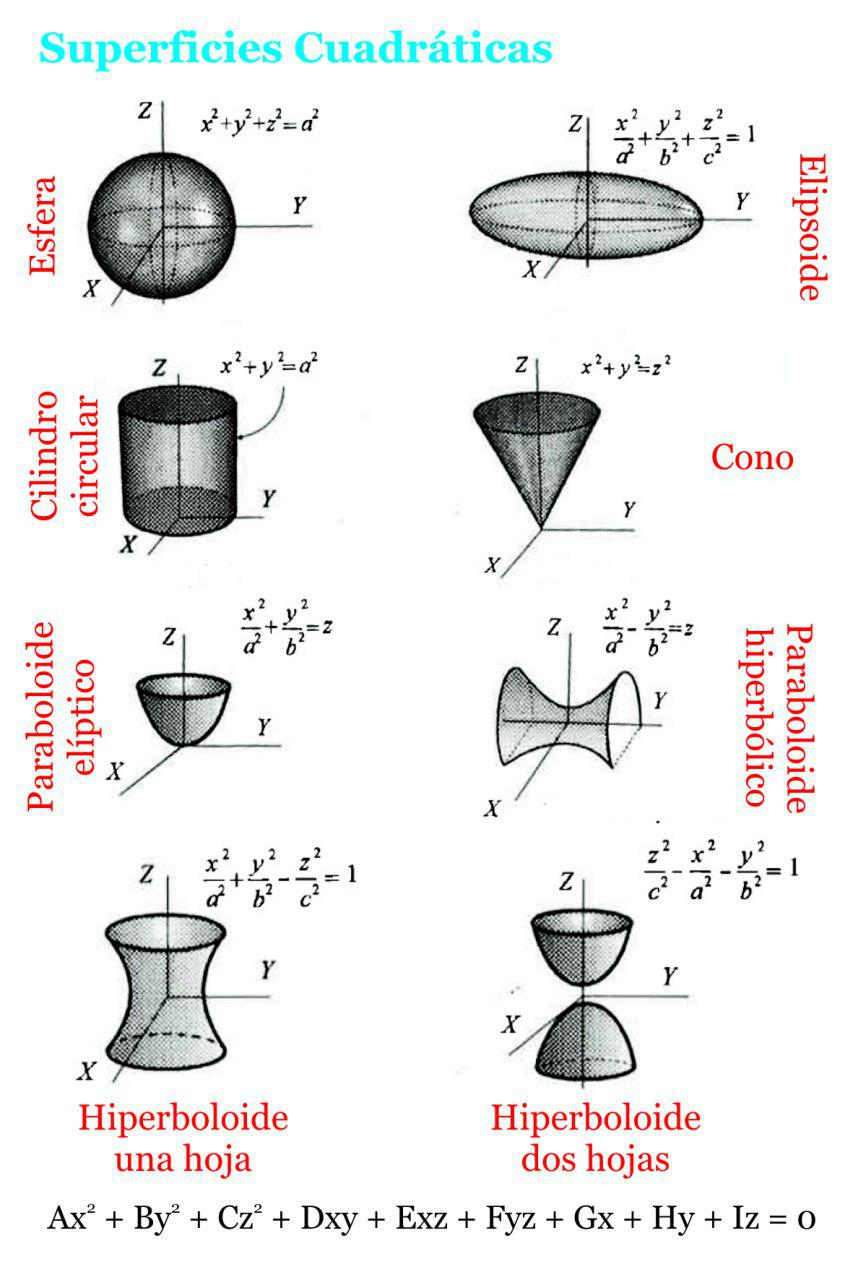
\includegraphics[width=0.87\linewidth]{./imagenes/cuadricas.jpg}
\end{figure}








\end{document}